\chapter{Folgen \& Konvergenz}


\setcounter{section}{4}
\setcounter{subsection}{0}
\setcounter{subsubsection}{1}
\setcounter{secnumdepth}{3}
\subsection{Zahlenfolgen }
\href{https://youtu.be/WS8kO3O_byk}{Video 02}\\
Definition:\\
Eine reele bzw. komplexe (Zahlen) Folge ist eine Funktion:\\
\begin{center}
	\boxed{x:\mathbb{N}\longmapsto \mathbb{R} (\text{ bzw.  }  \mathbb{C}) \text{ mit } n\longmapsto x_n} 
\end{center}
\begin{center}
	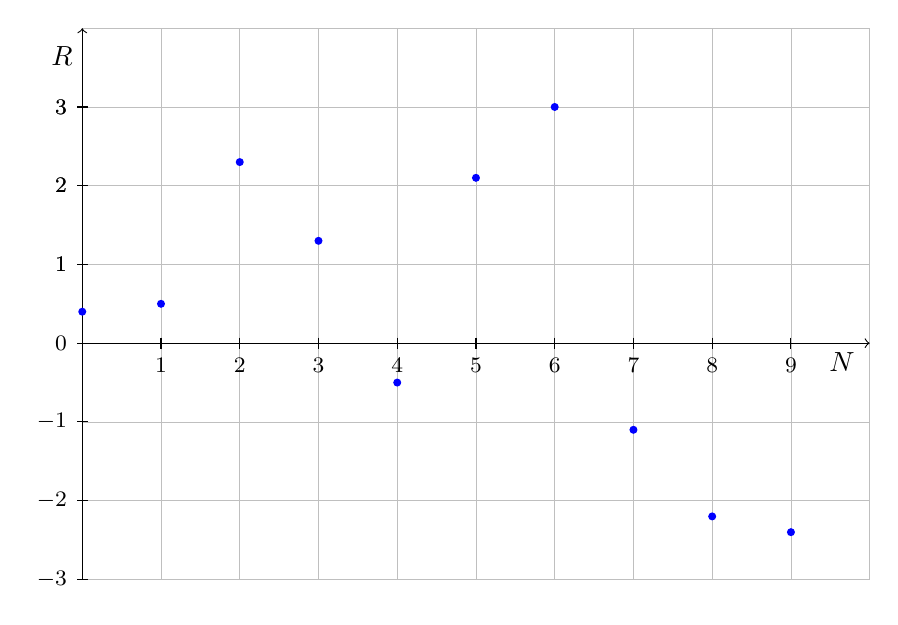
\begin{tikzpicture}
	%\filldraw [red,opacity=0.5] (0,0)--(-1,2)--(-2,4)--(-4,4)--(-4,0)--(0,0);
	% Gitternetzlinien
	\draw[xstep=1cm, ystep=1cm, very thin, color=lightgray] (0,-3) grid (10,4);
	% x-Achse
	\draw[->] (0,0) -- (10,0) node[below,xshift=-1em] {$\mathbb{N}$}; 
	%Zahlen auf x-Achse
	%\foreach \x in {-3,...,-1}
	%\draw[shift={(\x,0)},color=black] (0pt,2pt) -- (0pt,-2pt) node[below] {\footnotesize $\x$};
	\foreach \x in {1,...,9}
	\draw[shift={(\x,0)},color=black] (0pt,2pt) -- (0pt,-2pt) node[below] {\footnotesize $\x$};
	% y-Achse 
	\draw[->] (0,-3) -- (0,4) node[left,yshift=-1em] {$\mathbb{R}$};%node[above left]
	%Zahlen auf y-Achse
	\foreach \y in {-3,...,3}
	\draw[shift={(0,\y)},color=black] (2pt,0pt) -- (-2pt,0pt) node[left] {\footnotesize $\y$};
	\foreach \y in {1,...,3}
	\draw[shift={(0,\y)},color=black] (2pt,0pt) -- (-2pt,0pt) node[left] {\footnotesize $\y$};
	%Ursprung
	%\draw[color=black] (-1.5pt,-2pt) node[below] {\footnotesize $0$};
	
	%\draw[thick,color=black] plot[samples=200, domain=-2:0] 
	%(\x,{-2*\x}) node[below, xshift=-6.5em, yshift=9em] {$y=-2x$};
	
	
	
	\fill [blue] (0,0.4) circle (.051cm) ;	
	
	\fill [blue] (1,0.5) circle (.051cm) ;
	\fill [blue] (2,2.3) circle (.051cm) ;
	\fill [blue] (3,1.3) circle (.051cm) ;
	\fill [blue] (5,2.1) circle (.051cm) ;
	\fill [blue] (6,3) circle (.051cm) ;
	\fill [blue] (7,-1.1) circle (.051cm) ;
	\fill [blue] (8,-2.2) circle (.051cm) ;
	\fill [blue] (9,-2.4) circle (.051cm) ;	
	\fill [blue] (4,-0.5) circle (.051cm) ;	
	\end{tikzpicture}\\
\end{center}
Stattdessen schreibt man:\\
\begin{center}
	\boxed{x_0,x_1,x_2\ldots = (x_n)_{n\in \mathbb{N}}}
\end{center}
Beispiel:\vspace*{2mm}\\
\textbullet \;\; $ (\frac{1}{2^n})_{n\in \mathbb{N}}\; =1,\frac{1}{2},\frac{1}{4},\frac{1}{8}\ldots$\\
\newpage
\noindent
\textbullet \;\;$ (n^2)_{n\in \mathbb{N}} \;=0,1,4,9\ldots$\\
\begin{center}
	
	
	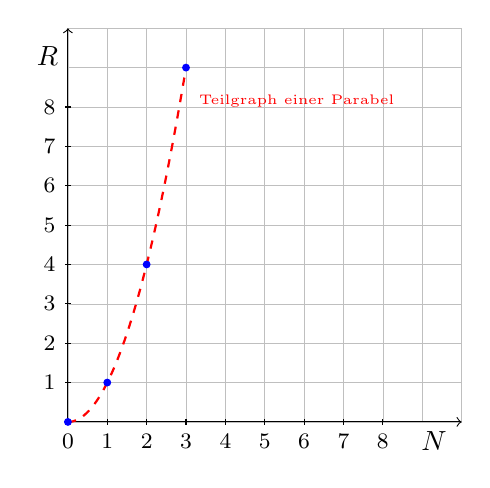
\begin{tikzpicture} [scale=0.5]
	
	% Gitternetzlinien
	\draw[xstep=1cm, ystep=1cm, very thin, color=lightgray] (0,0) grid (10,10);
	% x-Achse
	\draw[->] (0,0) -- (10,0) node[below,xshift=-1em] {$\mathbb{N}$}; 
	%Zahlen auf x-Achse
	%\foreach \x in {-3,...,-1}
	%\draw[shift={(\x,0)},color=black] (0pt,2pt) -- (0pt,-2pt) node[below] {\footnotesize $\x$};
	\foreach \x in {0,...,8}
	\draw[shift={(\x,0)},color=black] (0pt,2pt) -- (0pt,-2pt) node[below] {\footnotesize $\x$};
	% y-Achse 
	\draw[->] (0,0) -- (0,10) node[left,yshift=-1em] {$\mathbb{R}$};%node[above left]
	%Zahlen auf y-Achse
	%\foreach \y in {-1,...,-1}
	%\draw[shift={(0,\y)},color=black] (2pt,0pt) -- (-2pt,0pt) node[left] {\footnotesize $\y$};
	\foreach \y in {1,...,8}
	\draw[shift={(0,\y)},color=black] (2pt,0pt) -- (-2pt,0pt) node[left] {\footnotesize $\y$};
	%Ursprung
	%\draw[color=black] (0pt,-10pt) node[right] {\footnotesize $0$};
	
	\draw[thick,dashed,color=red] plot[samples=200, domain=0:3] 
	(\x,{\x*\x}) node[below, xshift=4em,yshift=-6] {\tiny{Teilgraph einer Parabel}};
	
	%\draw[thick,color=black] plot[samples=200, domain=-1:2] 
	%(\x,{\x-1}) node[below, xshift=1em]{$g(x)$};
	\fill [blue] (0,0) circle (.1cm) ;	
	\fill [blue] (1,1) circle (.1) ;
	\fill [blue] (2,4) circle (.1) ;
	\fill [blue] (3,9) circle (.1) ;
	%\fill [blue] (3,3) circle (.1cm) ;
	
	
	\end{tikzpicture}\\
\end{center}
\textbullet \;\; $(\frac{1}{n})_{n\in \mathbb{N}\backslash \{0\}} \;=1,\frac{1}{2} ,\frac{1}{3}\ldots$\vspace*{2mm}\\
\textbullet \;\; $ (1)_{n\in \mathbb{N}}=1,1,1,\ldots$\vspace*{2mm}\\
\textbullet \;\; $ (\mathrm{i}^n)_{n\in \mathbb{N}}\;=1,\mathrm{i},\mathrm{i}^2,\mathrm{i}^3,\mathrm{i}^4\ldots =\mathrm{i},-1,-\mathrm{i},1\ldots$
\subsection{Konvergenz von Zahlenfolgen }
\href{https://youtu.be/KBmVpgrY57o}{Video 03}\\
Definition:\\
Eine Folge $ (x_n)_{n\in \mathbb{N}} $ heißt konvergent gegen $ a\in\mathbb{R} $, wenn es zu jeden $ \varepsilon>0 $ ein $ n_0 $ gibt, s. d.\\
\begin{align*}
\boxed{
	|x_n-a|<\varepsilon \;\; \text{ für alle}\;\; n\geq n_0}
\end{align*}
gilt.\vspace*{2mm}\\
Wir schreiben dann:\\
\begin{align*}
\boxed{\lim\limits_ {n\to\infty}x_n=a}
\end{align*}
Eine Folge $ (x_n)_{n\in \mathbb{N}} $ heißt konvergent, wenn es ein $ a\in\mathbb{R} $ gibt, gegen das sie konvergiert.\\
Andersfall heißt $ (x_n)_{n\in \mathbb{N}} $ divergent.\\
\begin{center}
	
	
	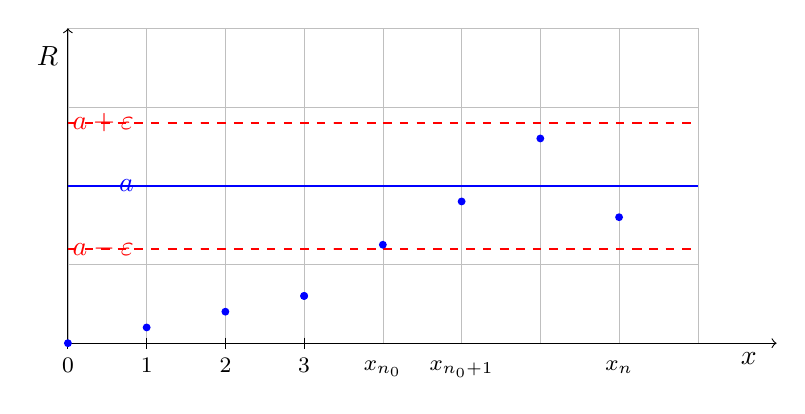
\begin{tikzpicture}
	
	% Gitternetzlinien
	\draw[xstep=1cm, ystep=1cm, very thin, color=lightgray] (0,0) grid (8,4);
	% x-Achse
	\draw[->] (0,0) -- (9,0) node[below,xshift=-1em] {$x$}; 
	%Zahlen auf x-Achse
	%\foreach \x in {-3,...,-1}
	%\draw[shift={(\x,0)},color=black] (0pt,2pt) -- (0pt,-2pt) node[below] {\footnotesize $\x$};
	\foreach \x in {0,...,3}
	\draw[shift={(\x,0)},color=black] (0pt,2pt) -- (0pt,-2pt) node[below] {\footnotesize $\x$};
	% y-Achse 
	\draw[->] (0,0) -- (0,4) node[left,yshift=-1em] {$\mathbb{R}$};%node[above left]
	%Zahlen auf y-Achse
	%\foreach \y in {-1,...,-1}
	%\draw[shift={(0,\y)},color=black] (2pt,0pt) -- (-2pt,0pt) node[left] {\footnotesize $\y$};
	%\foreach \y in {1,...,3}
	%\draw[shift={(0,\y)},color=black] (2pt,0pt) -- (-2pt,0pt) node[left] {\footnotesize $\y$};
	%Ursprung
	%\draw[color=black] (0pt,-10pt) node[right] {\footnotesize $0$};
	
	\draw[thick,color=red,dashed] plot[samples=200, domain=0:8] 
	(\x,{2.8}) node[left, xshift=-20em] {$a+\varepsilon$};
	\draw[thick,color=blue] plot[samples=200, domain=0:8] 
	(\x,{2}) node[left, xshift=-20em] {$a$};
	\draw[thick,color=red,dashed] plot[samples=200, domain=0:8] 
	(\x,{1.2}) node[left, xshift=-20em]{$a-\varepsilon$};
	
	\fill [blue] (0,0) circle (.05cm) ;	
	\fill [blue] (1,0.2) circle (.05) ;
	\fill [blue] (2,0.4) circle (.05) ;
	\fill [blue] (3,0.6) circle (.05) ;
	\fill [blue] (3,0.6) circle (.05) ;
	\fill [blue] (4,1.25) circle (.05) ;
	\fill [blue] (5,1.8) circle (.05) ;
	\fill [blue] (6,2.6) circle (0.05) ;
	\fill [blue] (7,1.6) circle (0.05) ;
	\draw[color=black] (4,-3pt) node[below] {\footnotesize $x_{n_0}$};
	\draw[color=black] (5,-3pt) node[below] {\footnotesize $x_{n_0+1}$};
	\draw[color=black] (7,-3pt) node[below] {\footnotesize $x_{n}$};
	\end{tikzpicture}\\
\end{center}
Ab den Wert $ n_0=4 $ sind alle Wert bis $ n $ im Bereich von $ a\pm \varepsilon $, dann konvergiert die Folge $ (x)_{n\in \mathbb{N}} $ gegen den Grenwert $ \lim\limits_ {n\to\infty}x_n=a $.\\
\subsubsection{Betrachtung der Folge $(\frac{1}{n})_{n\in \mathbb{N}\backslash\{0\}}  $}
\href{https://youtu.be/apfeLM-bE6A}{Video 04}\\
Betrachte die Folge $ (\frac{1}{n})_{n\in \mathbb{N}\backslash\{0\}}\;=1,\frac{1}{2},\frac{1}{3}\ldots $.\\
Wir wollen zeigen $ \lim\limits_ {n\to\infty}\frac{1}{n}=0 $.\vspace*{2mm}\\
Zu zeigen: Für jedes $ \varepsilon>0 $ gibt es ein $ n_0 \in \mathbb{N} $, s. d. $ |\frac{1}{n}-0|<\varepsilon $ für $ n\geq n_0 $.\\
Skizze:\\
\begin{center}
	\begin{tikzpicture}[yscale=3]
	
	% Gitternetzlinien
	\draw[xstep=1cm, ystep=0.3cm, very thin, color=lightgray] (0,-1) grid (8,1.2);
	% x-Achse
	\draw[->] (0,0) -- (8,0) node[below,xshift=-1em] {$\mathbb{N}$}; 
	%Zahlen auf x-Achse
	\foreach \x in {1,...,7}
	\draw[shift={(\x,0)},color=black] (0pt,2pt) -- (0pt,-2pt) node[below] {\footnotesize $\x$};
	%\foreach \x in {1,...,3}
	%\draw[shift={(\x,0)},color=black] (0pt,2pt) -- (0pt,-2pt) node[below] {\footnotesize $\x$};
	% y-Achse 
	\draw[->] (0,-1) -- (0,1.2) node[left,yshift=0em] {$\mathbb{R}$};%node[above left]
	%Zahlen auf y-Achse
	\foreach \y in {-1,...,-1}
	\draw[shift={(0,\y)},color=black] (2pt,0pt) -- (-2pt,0pt) node[left] {\footnotesize $\y$};
	\foreach \y in {1,...,1}
	\draw[shift={(0,\y)},color=black] (2pt,0pt) -- (-2pt,0pt) node[left] {\footnotesize $\y$};
	%Ursprung
	%\draw[color=black] (0pt,-10pt) node[right] {\footnotesize $0$};
	
	\draw[thick,color=red,dashed] plot[samples=200, domain=0:8] 
	(\x,{1/4}) node[left, xshift=-20em] {$\varepsilon=\genfrac{}{}{}{2}{1 }{4 }$};
	
	\draw[thick,color=red,dashed] plot[samples=200, domain=0:8] 
	(\x,{-1/4}) node[left, xshift=-20em]{$\varepsilon$};
	
	
	\draw[color=black] (1,1) node {\footnotesize \textbullet};
	\draw[color=black] (2,0.5) node {\footnotesize \textbullet};
	\draw[color=black] (3,0.33) node {\footnotesize \textbullet};
	\draw[color=black] (4,0.25) node {\footnotesize \textbullet};
	\draw[color=black] (5,0.2) node {\footnotesize \textbullet};
	\draw[color=black] (6,0.166) node {\footnotesize \textbullet};
	\draw[color=black] (7,0.142) node {\footnotesize \textbullet};
	\draw[color=black] (-1.5,0) node {\footnotesize Grenzwert=0};
	\draw[color=black] (5,-0.4) node {\footnotesize $ n_0=5 $};
	\end{tikzpicture}\\
\end{center}
Exemplarischen formalen Beweis von $ \lim\limits_ {n\to\infty}\frac{1}{n}=0 $.\\
Betrachte:\\
Sei $ \varepsilon>0 $ beliebig aber fest.
\begin{align}
&\bigg|\frac{1}{n}-0\bigg|=\bigg|\frac{1}{n}\bigg|=\frac{1}{n}<\varepsilon\\
&\Leftrightarrow \frac{1}{\varepsilon}<n
\end{align}
Wähle:\\
\begin{align*}
n_0=\bigg\lceil\frac{1}{\varepsilon}\bigg \rceil+1 \;\;\text{\tiny{aufgerundet $ \lceil0.7\rceil=1,\lceil2.1\rceil=3 $} }
\end{align*}
Dann gilt:\\
\begin{align*}
&n\geq n_0=\bigg\lceil\frac{1}{\varepsilon}\bigg\rceil+1\geq \frac{1}{\varepsilon}+1>\frac{1}{\varepsilon}\\
&\Leftrightarrow \frac{1}{\varepsilon} < n\\
&\Leftrightarrow\bigg|\frac{1}{n}-0\bigg|<\varepsilon_{\;\;_{\Square}} \;\;\;\;\text{wegen (IV.1), (IV.2)}\;\;\\
\end{align*}
\newpage
\noindent
\subsubsection{Beispiel für kovergente Folgen}
\href{https://youtu.be/qHlKFxy1ILw}{Video 06}\\
Zeige mit Hilfe der Definition der Konvergenz von Folgen, dass\\
\begin{align*}
\lim\limits_ {n\to\infty}\frac{1}{\sqrt[3]{n}}=0
\end{align*}
Zu zeigen:\\
Für $ \varepsilon>0 $ fest und beliebig exestiert ein $ n_0\in \mathbb{N}$, s.d. $\big |\frac{1}{\sqrt[3]{n}}\big|<\varepsilon $ für alle $ n>n_0 $\\
Betrachte:\\
\begin{align*}
&\bigg|\frac{1}{\sqrt[3]{n}}-0 \bigg |=\bigg |\frac{1}{\sqrt[3]{n}}\bigg |=\frac{1}{\sqrt[3]{n}}<\varepsilon\\
&\Leftrightarrow\frac{1}{\varepsilon}<\sqrt[3]{n}\\
&\Leftrightarrow \frac{1}{\varepsilon^3}<n\\
\end{align*}
Wähle:\\
\begin{align*}
n_0:=\bigg\lceil\frac{1}{\varepsilon^3}\bigg\rceil+1
\end{align*}
Dann gilt für alle:\\

\begin{align*}
n\geq n_0&\Leftrightarrow n\geq n_0=\bigg\lceil\frac{1}{\varepsilon^3}\bigg\rceil+1\geq\frac{1}{e^3}+1> \frac{1}{\varepsilon^3}_{_{\Square}}\\
& \Leftrightarrow \bigg |\frac{1}{\sqrt[3]{n}}-0 \bigg|<\varepsilon
\end{align*}
\subsection{Divergenz}
\href{https://youtu.be/r8IF-n0EyQg}{Video 07}\\
Eine Folge $(x_n)_{n\in\mathbb{N}}$ heißt divergent, wenn sie nicht konvergent ist.\vspace*{2mm}\\
Beispiel:\\
\textbullet \;\; $(n)_{n \in \mathbb{N}}=0,1,2,\ldots \lim\limits_ {n\to\infty}=\infty\;\;\;\;$\tiny{Bemerkung: $\infty\neq\mathbb{R}$} \\
\normalsize
\begin{center}
	
	
	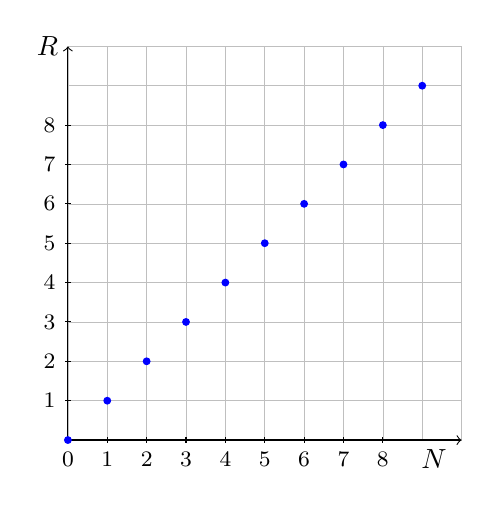
\begin{tikzpicture} [scale=0.5]
	
	% Gitternetzlinien
	\draw[xstep=1cm, ystep=1cm, very thin, color=lightgray] (0,0) grid (10,10);
	% x-Achse
	\draw[->] (0,0) -- (10,0) node[below,xshift=-1em] {$\mathbb{N}$}; 
	%Zahlen auf x-Achse
	%\foreach \x in {-3,...,-1}
	%\draw[shift={(\x,0)},color=black] (0pt,2pt) -- (0pt,-2pt) node[below] {\footnotesize $\x$};
	\foreach \x in {0,...,8}
	\draw[shift={(\x,0)},color=black] (0pt,2pt) -- (0pt,-2pt) node[below] {\footnotesize $\x$};
	% y-Achse 
	\draw[->] (0,0) -- (0,10) node[left,yshift=-0em] {$\mathbb{R}$};%node[above left]
	%Zahlen auf y-Achse
	%\foreach \y in {-1,...,-1}
	%\draw[shift={(0,\y)},color=black] (2pt,0pt) -- (-2pt,0pt) node[left] {\footnotesize $\y$};
	\foreach \y in {1,...,8}
	\draw[shift={(0,\y)},color=black] (2pt,0pt) -- (-2pt,0pt) node[left] {\footnotesize $\y$};
	%Ursprung
	%\draw[color=black] (0pt,-10pt) node[right] {\footnotesize $0$};
	
	%\draw[thick,dashed,color=red] plot[samples=200, domain=0:3] 
	%(\x,{\x*\x}) node[below, xshift=4em,yshift=-6] {\tiny{Teilgraph einer Parabel}};
	
	%\draw[thick,color=black] plot[samples=200, domain=-1:2] 
	%(\x,{\x-1}) node[below, xshift=1em]{$g(x)$}; 
	\fill [blue] (0,0) circle (.1cm) ;	
	\fill [blue] (1,1) circle (.1) ;
	\fill [blue] (2,2) circle (.1) ;
	\fill [blue] (3,3) circle (.1) ;
	
	\fill [blue] (4,4) circle (.1cm) ;	
	\fill [blue] (5,5) circle (.1) ;
	\fill [blue] (6,6) circle (.1) ;
	\fill [blue] (7,7) circle (.1) ;
	\fill [blue] (8,8) circle (.1) ;
	\fill [blue] (9,9) circle (.1) ;
	
	\end{tikzpicture}\\
\end{center}
\textbullet \;\; $ \big((-1)^n\big)_{n\in \mathbb{N}} =1,-1,1,-1,\ldots \lim\limits_ {n\to\infty}\big((-1)^n\big)$ exestiert nicht!\\

\begin{center}
	
	
	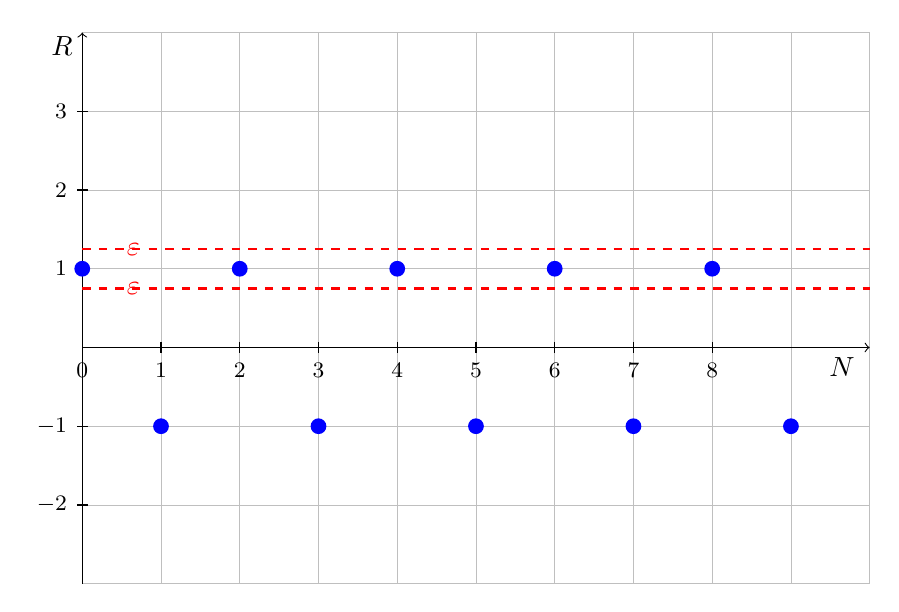
\begin{tikzpicture} [scale=1]
	
	% Gitternetzlinien
	\draw[xstep=1cm, ystep=1cm, very thin, color=lightgray] (0,-3) grid (10,4);
	% x-Achse
	\draw[->] (0,0) -- (10,0) node[below,xshift=-1em] {$\mathbb{N}$}; 
	%Zahlen auf x-Achse
	%\foreach \x in {-3,...,-1}
	%\draw[shift={(\x,0)},color=black] (0pt,2pt) -- (0pt,-2pt) node[below] {\footnotesize $\x$};
	\foreach \x in {0,...,8}
	\draw[shift={(\x,0)},color=black] (0pt,2pt) -- (0pt,-2pt) node[below] {\footnotesize $\x$};
	% y-Achse 
	\draw[->] (0,-3) -- (0,4) node[left,yshift=-0.5em] {$\mathbb{R}$};%node[above left]
	%Zahlen auf y-Achse
	\foreach \y in {-2,...,-1}
	\draw[shift={(0,\y)},color=black] (2pt,0pt) -- (-2pt,0pt) node[left] {\footnotesize $\y$};
	\foreach \y in {1,...,3}
	\draw[shift={(0,\y)},color=black] (2pt,0pt) -- (-2pt,0pt) node[left] {\footnotesize $\y$};
	%Ursprung
	%\draw[color=black] (0pt,-10pt) node[right] {\footnotesize $0$};
	
	%\draw[thick,dashed,color=red] plot[samples=200, domain=0:3] 
	%(\x,{\x*\x}) node[below, xshift=4em,yshift=-6] {\tiny{Teilgraph einer Parabel}};
	
	%\draw[thick,color=black] plot[samples=200, domain=-1:2] 
	%(\x,{\x-1}) node[below, xshift=1em]{$g(x)$}; 
	\fill [blue] (0,1) circle (.1cm) ;	
	\fill [blue] (1,-1) circle (.1) ;
	\fill [blue] (2,1) circle (.1) ;
	\fill [blue] (3,-1) circle (.1) ;
	
	\fill [blue] (4,1) circle (.1cm) ;	
	\fill [blue] (5,-1) circle (.1) ;
	\fill [blue] (6,1) circle (.1) ;
	\fill [blue] (7,-1) circle (.1) ;
	\fill [blue] (8,1) circle (.1) ;
	\fill [blue] (9,-1) circle (.1) ;
	\draw[thick,color=red,dashed] plot[samples=200, domain=0:10] 
	(\x,{3/4}) node[left, xshift=-26em]{$\varepsilon$};
	\draw[thick,color=red,dashed] plot[samples=200, domain=0:10] 
	(\x,{5/4}) node[left, xshift=-26em]{$\varepsilon$};
	\end{tikzpicture}\\
\end{center}
Bei jedem $ \varepsilon $ muß gelten, dass alle Werte größer $ n_0 $ im $ \varepsilon $-Bereich sein mussen. Dies ist hier nicht gegeben. Diese Folge hat keinen Grenzwert.\vspace*{2mm}\\
\textbullet \;\; $ (-n)_{n\in \mathbb{N}} =0,-1,-2,\ldots \lim\limits_ {n\to\infty}=-\infty$\\
\begin{center}
	
	
	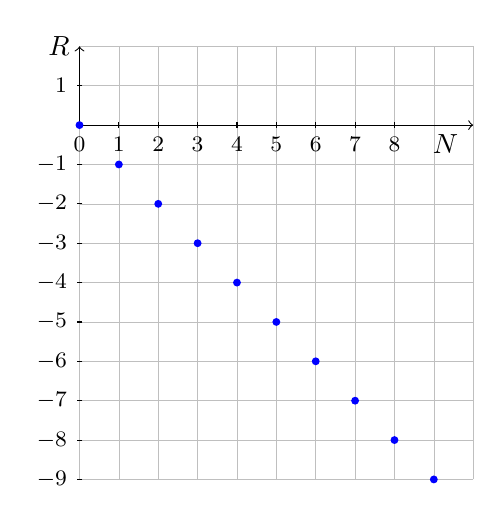
\begin{tikzpicture} [scale=0.5]
	
	% Gitternetzlinien
	\draw[xstep=1cm, ystep=1cm, very thin, color=lightgray] (0,-9) grid (10,2);
	% x-Achse
	\draw[->] (0,0) -- (10,0) node[below,xshift=-1em] {$\mathbb{N}$}; 
	%Zahlen auf x-Achse
	%\foreach \x in {-3,...,-1}
	%\draw[shift={(\x,0)},color=black] (0pt,2pt) -- (0pt,-2pt) node[below] {\footnotesize $\x$};
	\foreach \x in {0,...,8}
	\draw[shift={(\x,0)},color=black] (0pt,2pt) -- (0pt,-2pt) node[below] {\footnotesize $\x$};
	% y-Achse 
	\draw[->] (0,0) -- (0,2) node[left,yshift=0em] {$\mathbb{R}$};%node[above left]
	%Zahlen auf y-Achse
	\foreach \y in {-9,...,-1}
	\draw[shift={(0,\y)},color=black] (2pt,0pt) -- (-2pt,0pt) node[left] {\footnotesize $\y$};
	\foreach \y in {1,...,1}
	\draw[shift={(0,\y)},color=black] (2pt,0pt) -- (-2pt,0pt) node[left] {\footnotesize $\y$};
	%Ursprung
	%\draw[color=black] (0pt,-10pt) node[right] {\footnotesize $0$};
	
	%\draw[thick,dashed,color=red] plot[samples=200, domain=0:3] 
	%(\x,{\x*\x}) node[below, xshift=4em,yshift=-6] {\tiny{Teilgraph einer Parabel}};
	
	%\draw[thick,color=black] plot[samples=200, domain=-1:2] 
	%(\x,{\x-1}) node[below, xshift=1em]{$g(x)$}; 
	\fill [blue] (0,0) circle (.1cm) ;	
	\fill [blue] (1,-1) circle (.1) ;
	\fill [blue] (2,-2) circle (.1) ;
	\fill [blue] (3,-3) circle (.1) ;
	
	\fill [blue] (4,-4) circle (.1cm) ;	
	\fill [blue] (5,-5) circle (.1) ;
	\fill [blue] (6,-6) circle (.1) ;
	\fill [blue] (7,-7) circle (.1) ;
	\fill [blue] (8,-8) circle (.1) ;
	\fill [blue] (9,-9) circle (.1) ;
	
	\end{tikzpicture}\\
\end{center}
Definition: (Bestimmte Divergenz)\\
Eine Folge $ (x_n)_{n\in \mathbb{N}} $ ist bestimmt divergent gegen $ +\infty $ bzw. $ -\infty $, wenn zu jedem $ \varepsilon>0 $ ein $ n_0\in\mathbb{N} $ exestiert mit der Eigenschaft s.d. gilt:\\
.
\begin{center}
	\fbox{\parbox  {38mm} {
			$x_n>\varepsilon\; \;\;\;\;\text{für } n>n_0$\\
			$x_n<-\varepsilon \;\;\text{für } n>n_0$}}
\end{center}

\begin{center}
	
	
	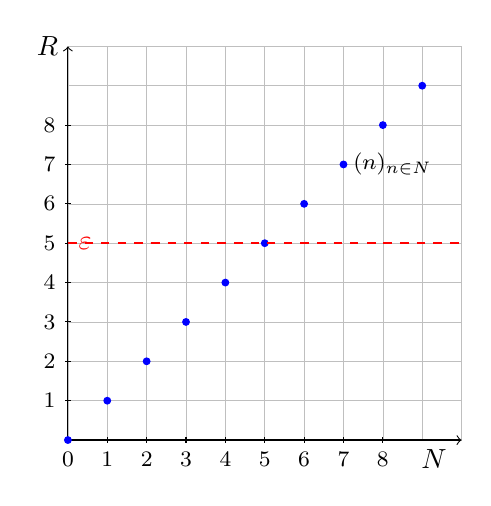
\begin{tikzpicture} [scale=0.5]
	
	% Gitternetzlinien
	\draw[xstep=1cm, ystep=1cm, very thin, color=lightgray] (0,0) grid (10,10);
	% x-Achse
	\draw[->] (0,0) -- (10,0) node[below,xshift=-1em] {$\mathbb{N}$}; 
	%Zahlen auf x-Achse
	%\foreach \x in {-3,...,-1}
	%\draw[shift={(\x,0)},color=black] (0pt,2pt) -- (0pt,-2pt) node[below] {\footnotesize $\x$};
	\foreach \x in {0,...,8}
	\draw[shift={(\x,0)},color=black] (0pt,2pt) -- (0pt,-2pt) node[below] {\footnotesize $\x$};
	% y-Achse 
	\draw[->] (0,0) -- (0,10) node[left,yshift=-0em] {$\mathbb{R}$};%node[above left]
	%Zahlen auf y-Achse
	%\foreach \y in {-1,...,-1}
	%\draw[shift={(0,\y)},color=black] (2pt,0pt) -- (-2pt,0pt) node[left] {\footnotesize $\y$};
	\foreach \y in {1,...,8}
	\draw[shift={(0,\y)},color=black] (2pt,0pt) -- (-2pt,0pt) node[left] {\footnotesize $\y$};
	%Ursprung
	%\draw[color=black] (0pt,-10pt) node[right] {\footnotesize $0$};
	
	%\draw[thick,dashed,color=red] plot[samples=200, domain=0:3] 
	%(\x,{\x*\x}) node[below, xshift=4em,yshift=-6] {\tiny{Teilgraph einer Parabel}};
	
	%\draw[thick,color=black] plot[samples=200, domain=-1:2] 
	%(\x,{\x-1}) node[below, xshift=1em]{$g(x)$}; 
	\fill [blue] (0,0) circle (.1cm) ;	
	\fill [blue] (1,1) circle (.1) ;
	\fill [blue] (2,2) circle (.1) ;
	\fill [blue] (3,3) circle (.1) ;
	
	\fill [blue] (4,4) circle (.1cm) ;	
	\fill [blue] (5,5) circle (.1) ;
	\fill [blue] (6,6) circle (.1) ;
	\fill [blue] (7,7) circle (.1) ;
	\fill [blue] (8,8) circle (.1) ;
	\fill [blue] (9,9) circle (.1) ;
	\draw[thick,color=red,dashed] plot[samples=200, domain=0:10] 
	(\x,{5}) node[left, xshift=-13em]{$\varepsilon$};
	\draw[color=black] (7,7) node[right] {\footnotesize $(n)_{n\in\mathbb{N}}$};
	\end{tikzpicture}\\
\end{center}
\subsection{Rechenregeln für konvergente Folgen}
\href{https://youtu.be/m6GeFKpvFQ8}{Video 08}\\
\href{https://youtu.be/wWXpWP5EGCU}{Video 09}\\
Berechnung von Grenzwerten:\\
Beispiel:\\
\textbullet \;\; $ 0=\lim\limits_ {n\to\infty}\bigg(\frac{1}{n}\cdot \frac{1}{n}\bigg)=\lim\limits_ {n\to\infty}\bigg(\frac{1}{n}\bigg)\cdot\lim\limits_ {n\to\infty}\bigg(\frac{1}{n}\bigg)=0\cdot 0=0 $\\
\textbullet \;\; $ 1=\lim\limits_ {n\to\infty}1 =\lim\limits_ {n\to\infty}\bigg(n\cdot \frac{1}{n}\bigg)\overset{falsch}{=}\lim\limits_ {n\to\infty} n\cdot \lim\limits_ {n\to\infty}\bigg(\frac{1}{n}\bigg)=0\cdot\infty=0 $ \text{ falsch!!}\vspace*{4mm}\\
Nicht definiert und falsch ist:\\
\begin{align*}
&0\cdot\infty\\
&\frac{1}{\infty}=0\\
&\text{mit }\;\;\infty\;\; \text{kann man nicht rechnen! }
\end{align*}\vspace*{2mm}\\
\textbf{Rechenregeln für konvergente Folgen:}\\
Seien $ (x_n)_{n\in\mathbb{N}} $,$ (y_n)_{y\in \mathbb{N}} $ konvergente Folgen mit:\\
\begin{align*}
\lim\limits_ {n\to\infty}x_n=a \;\;\text{und }\;\; \lim\limits_ {n\to\infty}y_n=b\;\;\text{sowie }c\in \mathbb{R}
\end{align*}
dann gilt:\\
\begin{center}
	
	\fbox{\parbox  {98mm} {
			\begin{align*}
			1.&\lim\limits_ {n\to\infty}(x_n+y_n)=a+b\\
			2.&\lim\limits_ {n\to\infty}(x_n\cdot y_n)=a\cdot b\\
			3.&\lim\limits_ {n\to\infty}(c\cdot x_n)=c\cdot a\\
			4.&\lim\limits_ {n\to\infty}\bigg(\frac{x_n}{y_n}\bigg)=\frac{a}{b}\;\; \text{falls } b\neq 0\neq y_n\;\;\text{für alle }\;\;n\in \mathbb{N}\\
			5.&\; a\leq b\;\;\text{falls }\;\;x_n\leq y_n\;\;\text{für alle }\;\;n\in\mathbb{N}
			\end{align*}}}
\end{center}
\textbullet \;\; zu 1. :\\
\begin{align*}
\lim\limits_ {n\to\infty}\bigg(\frac{1}{n}+\frac{1}{n^2}\bigg)=\lim\limits_ {n\to\infty}\bigg(\frac{1}{n}\bigg)+\lim\limits_ {n\to\infty}\bigg(\frac{1}{n^2}\bigg)=0+0=0
\end{align*}
\textbullet \;\; zu 2. :\\
\begin{align*}
\lim\limits_ {n\to\infty}\bigg(\frac{1}{n}\cdot \frac{1}{n}\bigg)=\lim\limits_ {n\to\infty}\bigg(\frac{1}{n}\bigg)\cdot\lim\limits_ {n\to\infty}\bigg(\frac{1}{n}\bigg)=0\cdot 0=0\\
\end{align*}
\textbullet \;\; zu 3. :\\
\begin{align*}
\lim\limits_ {n\to\infty}\bigg(7\cdot\frac{1}{n^2}\bigg)=7\cdot \lim\limits_ {n\to\infty}\bigg(\frac{1}{n^2}\bigg)=7\cdot0 =0
\end{align*}
\textbullet \;\; zu 4. :\\
\begin{align*}
\lim\limits_ {n\to\infty}\Biggr(\frac{\lim\limits_ {n\to\infty}\frac{1}{n}}{\lim\limits_ {n\to\infty}\frac{1}{n^2}+1}\Bigg)=\Bigg(\frac{\lim\limits_ {n\to\infty}\frac{1}{n}}{\lim\limits_ {n\to\infty}\frac{1}{n^2}+\lim\limits_ {n\to\infty}1}\Bigg)=\frac{0}{0+1}=0
\end{align*}
\textbullet \;\; zu 5. :\\
\begin{align*}
\lim\limits_ {n\to\infty}\bigg|\frac{\cos(n)}{n}\bigg|\;\;\text{für }\;\;n>0
\end{align*}
Suche Folgen $ a,b,c $ für die gilt:\\
\begin{align*}
&a\leq b \leq c \;\;\text{falls }\;\; x_n\leq y_n \leq z_n \;\; \text{für alle }\;\;n\in \mathbb{N}\backslash {0}\\
&a=0\;\; \text{weil }\;\;0<\bigg|\frac{\cos(n)}{n}\bigg|\;\text{für }\;\;n>0\\
&b=\lim\limits_ {n\to\infty}\bigg|\frac{\cos(x)}{n}\bigg|\\
&c=\lim\limits_ {n\to\infty}\frac{1}{n}>\lim\limits_ {n\to\infty}\bigg|\frac{\cos(n)}{n}\bigg|
\end{align*}
$\bigg|\frac{\cos(n)}{n}\bigg|<\frac{1}{n}  $ weil:\\
\begin{align*}
0<|\cos(n)|<1
\end{align*}
\begin{center}
	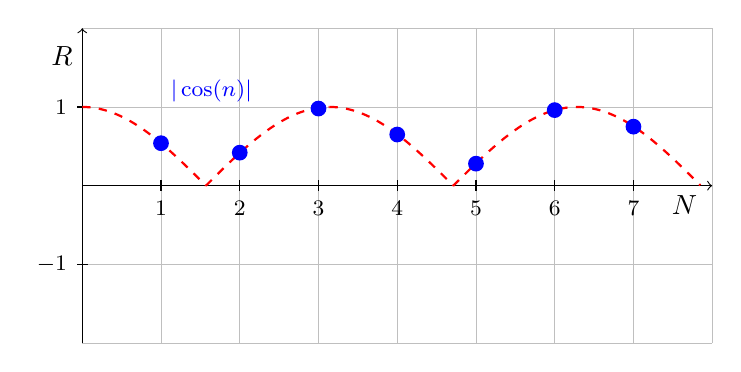
\begin{tikzpicture}
	
	% Gitternetzlinien
	\draw[xstep=1cm, ystep=1cm, very thin, color=lightgray] (0,-2) grid (8,2);
	% x-Achse
	\draw[->] (0,0) -- (8,0) node[below,xshift=-1em] {$\mathbb{N}$}; 
	%Zahlen auf x-Achse
	\foreach \x in {1,...,7}
	\draw[shift={(\x,0)},color=black] (0pt,2pt) -- (0pt,-2pt) node[below] {\footnotesize $\x$};
	%\foreach \x in {1,...,3}
	%\draw[shift={(\x,0)},color=black] (0pt,2pt) -- (0pt,-2pt) node[below] {\footnotesize $\x$};
	% y-Achse 
	\draw[->] (0,-2) -- (0,2) node[left,yshift=-1em] {$\mathbb{R}$};%node[above left]
	%Zahlen auf y-Achse
	\foreach \y in {-1,...,-1}
	\draw[shift={(0,\y)},color=black] (2pt,0pt) -- (-2pt,0pt) node[left] {\footnotesize $\y$};
	\foreach \y in {1,...,1}
	\draw[shift={(0,\y)},color=black] (2pt,0pt) -- (-2pt,0pt) node[left] {\footnotesize $\y$};
	%Ursprung
	%\draw[color=black] (0pt,-10pt) node[right] {\footnotesize $0$};
	\draw[thick,color=red,dashed] plot[samples=200, domain=0:3.14/2] 
	(\x,{cos(\x r)});
	\draw[thick,color=red,dashed] plot[samples=200, domain=3.14/2:3.14] 
	(\x,{abs(cos(\x r))});
	\draw[thick,color=red,dashed] plot[samples=200, domain=3.14:(3.14+3.14/2)] 
	(\x,{abs(cos(\x r))});
	\draw[thick,color=red,dashed] plot[samples=200, domain=(3.14+3.14/2):(3.14+3.14/2+3.14)] 
	(\x,{cos(\x r)});
	%\draw[thick,color=black] plot[samples=200, domain=-1:2] 
	%(\x,{\x-1}) node[below, xshift=1em]{$g(x)$};
	\fill [blue] (1,0.54) circle (.1cm) ;	
	\fill [blue] (2,0.42) circle (.1) ;
	\fill [blue] (3,0.98) circle (.1) ;
	\fill [blue] (4,0.65) circle (.1) ;
	\fill [blue] (5,0.28) circle (.1) ;
	\fill [blue] (6,0.96) circle (.1) ;
	\fill [blue] (7,0.75) circle (.1) ;
	\draw[color=blue] (1,1.2) node[right] {\footnotesize $|\cos(n)|$};
	\end{tikzpicture}\\
\end{center}
dann gilt:\\
\begin{align*}
&\lim\limits_ {n\to\infty} a\leq \lim\limits_ {n\to\infty} b\leq \lim\limits_ {n\to\infty} c\\
&\lim\limits_ {n\to\infty}0\leq\lim\limits_ {n\to\infty}\bigg|\frac{\cos(n)}{n}\bigg|\leq\lim\limits_ {n\to\infty}\frac{1}{n}\\
&0\leq\lim\limits_ {n\to\infty}\bigg|\frac{\cos(n)}{n}\bigg|\leq0\\
&\Rightarrow\lim\limits_ {n\to\infty}\bigg|\frac{\cos(n)}{n}\bigg|=0
\end{align*}
\newpage
\noindent
\subsubsection{Tricks zur Berechnung von Grenzwerten I}
\href{https://youtu.be/4DUydSPIVLM}{Video 10}\\
Berechne (falls exestieren) die folgenden Grenzwerte:\\
\begin{align*}
(i)&\lim\limits_ {n\to\infty}\bigg(\frac{n^5+7n}{3n^5+7n^4}\bigg)\\
(ii)&\lim\limits_ {n\to\infty}\bigg(\frac{n^2+4n}{n^3-2n^2}-7n^4\bigg)
\end{align*}
zu(i)$ \;\;\lim\limits_ {n\to\infty}\big(\frac{n^5+7n}{3n^5+7n^4}\big)\\ $
\begin{quote}
	NR:\\
	Man schaut sich die höchsten n- Potenzen vom Zähler und Nenner an.\\
	\begin{align*}
	\lim\limits_ {n\to\infty}\frac{n^5}{3n^5}=\lim\limits_ {n\to\infty} \frac{1}{3}=\frac{1}{3}\\ 
	\end{align*}
	Dies ist nur eine Überlegung und kein Beweis!\\
	\begin{align*}
	\lim\limits_ {n\to\infty}\bigg(\frac{n^5+7n}{3n^5+7n^4}\bigg)=\lim\limits_ {n\to\infty}\bigg(\frac{n^5(1+\frac{7}{n^4})}{n^5(1+\frac{7}{n})}\bigg)=\frac{\lim\limits_ {n\to\infty} 1+\frac{7}{n^4}}{\lim\limits_ {n\to\infty}3+\frac{7}{n}}=\frac{1+0}{3+0}=\frac{1}{3}\\
	\end{align*}
\end{quote}
zu(ii)\;\;$\lim\limits_ {n\to\infty}\big(\frac{n^2+4n}{n^3-2n^2}-7n^4\big)  $\\
\begin{quote}
	Die Rechenregeln für konvergente Folgen kann hier nicht angewendet werden, weil $ -7n^4 $ divergent ist.\\
	Da der Grenzwert von $ \lim\limits_ {n\to\infty}-7n^4=-\infty $ ist, divergiert diese Folge.\\
	\begin{align*}
	\lim\limits_ {n\to\infty}\bigg(\frac{n^2+4n}{n^3-2n^2}-7n^4\bigg)=-\infty
	\end{align*}
	Auch die Überlegung mit den n-Potenzen ergibt:\\
	NR:\\
	\begin{align*}
	\frac{n^2+4n}{n^3-2n^2}-7n=\frac{n^2+4n-(n^3-2n^2)7n}{n^3-2n^2}=\frac{n^2+4-7n^4+14n^3}{n^3-2n^2}
	\end{align*}
	Die höchsten n-Potenzen sind:\\
	\begin{align*}
	\frac{-7n^4}{n^3}=-7n\\
	\lim\limits_ {n\to\infty}-7n=-\infty
	\end{align*}
\end{quote}
\subsubsection{Tricks zur Berechnung von Grenzwerten II}
\href{https://youtu.be/3wf0Q-vtFGo}{Video 11}\\
Berechne (falls exestieren) die folgenden Grenzwerte:\\
\begin{tabular}[t]{lll}% l=linksbündig r=rechtsbündig
	(i) & $\lim\limits_ {n\to\infty}\frac{n^2}{\sqrt{n^5-n}} \;\;\text{für }\;\; n>0   $ \vspace*{2mm} \\
	(ii) & $\lim\limits_ {n\to\infty}\frac{-1^n}{n}\;\;\text{für }\;\; n>0  $\vspace*{2mm}  \\	
	(iii)&$\lim\limits_ {n\to\infty}\frac{cos(n)}{n}\;\;\text{für }\;\; n>0  \vspace*{4mm}$
\end{tabular} \\
Zu (i):\\
\begin{quote}
	\begin{align*}
	\lim\limits_ {n\to\infty}\frac{n^2}{\sqrt{n^5-n}} \;\;\text{für }\;\; n>0 
	\end{align*}
	Der Grenzwert, mit den höchsten n-Potenzen ist $ \approx \lim\limits_ {n\to\infty}\frac{n^2}{\sqrt[2]{n^5}}$ \\
	\begin{align*}
	\lim\limits_ {n\to\infty}\frac{2}{\sqrt[2]{n^5}}=\frac{n^2}{n^{\frac{5}{2}}}=n^2 n^{-\frac{5}{2}}=n^{-\frac{1}{2}}=\frac{1}{\sqrt{n}}=0
	\end{align*}
	Mit Berechnung ergibt sich:\\
	\begin{align*}
	&\lim\limits_ {n\to\infty}\frac{n^2}{\sqrt{n^5-n}} =\frac{n^2}{\sqrt{n^5(1-\frac{1}{n^4})}}=\frac{n^2}{\sqrt{n^5}}\frac{1}{\sqrt{1-\frac{1}{n^4}}}=\frac{n^2}{n^{\frac{5}{2}}}
	\frac{1}{\sqrt{1-\frac{1}{n^4}}}=\lim\limits_ {n\to\infty}\frac{1}{\sqrt{n}}\frac{1}{\lim\limits_ {n\to\infty}\sqrt{1-\frac{1}{n^4}}}=0\cdot 1=0\\
	&\lim\limits_ {n\to\infty}\frac{n^2}{\sqrt{n^5-n}}=0
	\end{align*}
\end{quote}
zu (ii):\\
\begin{quote}
	\begin{align*}
	\lim\limits_ {n\to\infty}\frac{-1^n}{n}\;\;\text{für }\;\;n>0
	\end{align*}
	Der Grenzwert von$\lim\limits_ {n\to\infty}-1^n  $ exestiert nicht, deswegen sind die Rechenregeln nicht anwendbar.\\
	Es gilt:\\
	\begin{align*}
	\frac{-1}{n}\leq\frac{-1^n}{n}\leq \frac{1}{n}
	\end{align*}
	Ebenso gilt auch:\\
	\begin{align*}
	\lim\limits_ {n\to\infty}\frac{-1}{n}&\leq \lim\limits_ {n\to\infty}\frac{-1^n}{n}\leq \lim\limits_ {n\to\infty}\frac{1}{n}\\
	0&\leq\lim\limits_ {n\to\infty}\frac{-1^n}{n}\leq 0
	\end{align*}
	Daraus folgt nach dem Quetschlemma:\\
	\begin{align*}
	\lim\limits_ {n\to\infty}\frac{-1^n}{n}=0
	\end{align*}
\end{quote}
zu (iii):\\
\begin{quote}
	\begin{align*}
	\lim\limits_ {n\to\infty}\frac{cos(n)}{n}\;\;\text{für }\;\; n>0 
	\end{align*}
	Es gilt für $ cos(n) $:\\
	\begin{align*}
	-1<cos(n)<1
	\end{align*}
	Ebenso gilt:\\
	\begin{align*}
	\frac{-1}{n}<\frac{cos(n)}{n}<\frac{1}{n}\\
	\end{align*}
	Daraus folgt:\\
	\begin{align*}
	\lim\limits_ {n\to\infty} \frac{-1}{n}&<\lim\limits_ {n\to\infty}\frac{cos(n)}{n}<\lim\limits_ {n\to\infty}\frac{1}{n}\\
	0&<\lim\limits_ {n\to\infty}\frac{cos(x)}{n}<0
	\end{align*}
	Und nach dem Quetschlemma gilt:\\
	\begin{align*}
	\lim\limits_ {n\to\infty}\frac{cos(n)}{n}=0
	\end{align*}	
\end{quote}
\subsubsection{Tricks zur Berechnung von Grenzwerten III}
\href{https://youtu.be/KqTM73LzkMo}{Video 12}\\
Berechne (falls exestieren) die folgenden Grenzwerte:\\
\begin{align*}
\lim\limits_ {n\to\infty}\sqrt{n^2+n+2}-\sqrt{n^2+2}
\end{align*}
Mit Hilfe der 3. Binomischen Formel erzeugt man einen Bruch:\\
\begin{align*}
&a^2-b^2=(a-b)(a+b)\\
&a-b=\frac{(a-b)(a+b)}{(a+b)}=\frac{a^2-b^2}{(a+b)}
\end{align*}
\begin{align*}
\lim\limits_ {n\to\infty} \underbrace {\sqrt{n^2+n+2}}_{a}-\underbrace {\sqrt{n^2+2}}_{b}=\frac{(n^2+n+2)-(n^2+2)}{\sqrt{n^2+n+2}+\sqrt{n^2+2}}=\frac{n}{\sqrt{n^2+n+2}+\sqrt{n^2+2}}
\end{align*}
Der Grenzwert, mit den höchsten n-Potenzen ist $ \approx \lim\limits_ {n\to\infty}\frac{n}{\sqrt{n^2}+\sqrt{n^2}}$ \\
\begin{align*}
\lim\limits_ {n\to\infty}\frac{n}{\sqrt{n^2}+\sqrt{n^2}}=\frac{n}{n+n}=\frac{n}{2n}=\frac{1}{2}
\end{align*}
Mit Berechnung ergibt sich:\\
\begin{align*}
\lim\limits_ {n\to\infty}\frac{n}{\sqrt{n^2+n+2}+\sqrt{n^2+2}}&=\frac{n}{\sqrt{n^2(1+\frac{1}{n}+\frac{2}{n^2})}+\sqrt{n^2(1+\frac{2}{n^2})}}\\
&=\frac{n}{n\bigg(\sqrt{1+\frac{1}{n}+\frac{2}{n^2}}\bigg)+\bigg(\sqrt{1+\frac{2}{n^2}}\bigg)}\\
&=\frac{1}{\sqrt{1+\frac{1}{n}+\frac{2}{n^2}}+\sqrt{1+\frac{2}{n^2}}}\\
&=\lim\limits_ {n\to\infty}\frac{1}{\sqrt{1+\frac{1}{n}+\frac{2}{n^2}}+\sqrt{1+\frac{2}{n^2}}}=\frac{1}{\sqrt{1+0+0}+\sqrt{1+0}}=\frac{1}{\sqrt{1}+\sqrt{1}}=\frac{1}{2}\\
\end{align*}
Dann ist der Grenzwert von:\\
\begin{align*}
\lim\limits_ {n\to\infty}\sqrt{n^2+n+2}-\sqrt{n^2+2}=\frac{1}{2}
\end{align*}
\subsection{Monotonie von Folgen}
\href{https://youtu.be/W9Xl_hHf18I}{Video 13}\\
Definition:\\
Eine reelle Folge $ (x)_{n\in\mathbb{N}} $ heißt streng monoton wachsend wenn gilt:\\
\begin{align*}
x_n< x_n+1\;\;\text{für alle }\;\; n\in \mathbb{N}\\  
\end{align*}
Eine reelle Folge $ (x)_{n\in\mathbb{N}} $ heißt streng monoton fallend wenn gilt:\\
\begin{align*}
x_n>x_n+1\;\;\text{für alle }\;\; n\in \mathbb{N}\\  
\end{align*}
Eine reelle Folge $ (x)_{n\in\mathbb{N}} $ heißt monoton wachsend wenn gilt:\\
\begin{align*}
x_n\leq x_n+1\;\;\text{für alle }\;\; n\in \mathbb{N}\\  
\end{align*}
Eine reelle Folge $ (x)_{n\in\mathbb{N}} $ heißt  monoton fallend wenn gilt:\\
\begin{align*}
x_n\geq x_n+1\;\;\text{für alle }\;\; n\in \mathbb{N}\\  
\end{align*}
\newpage
\noindent
\begin{center}
	Streng monoton wachsende Folge $ (x)_{n\in\mathbb{N}}$\\
	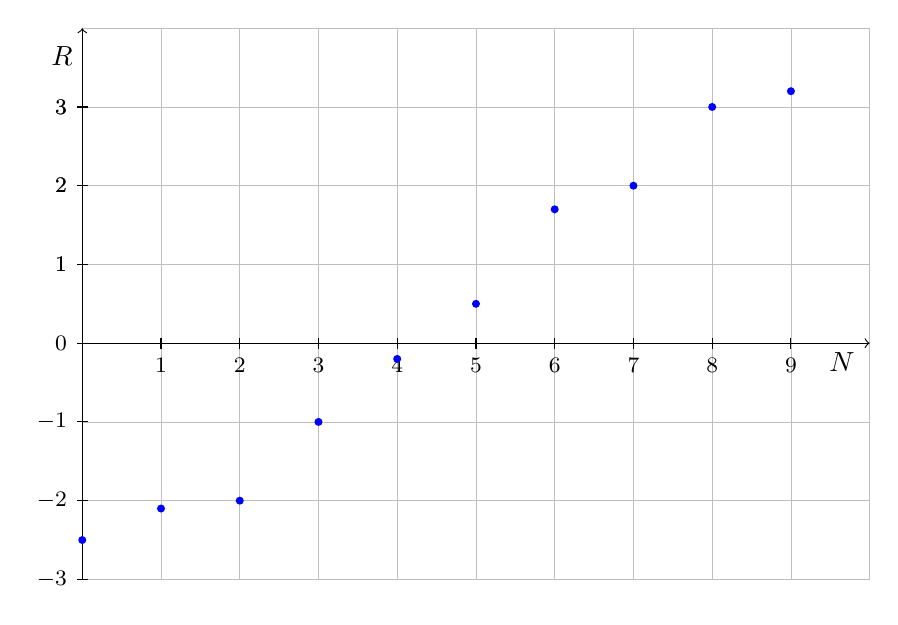
\begin{tikzpicture}
	%\filldraw [red,opacity=0.5] (0,0)--(-1,2)--(-2,4)--(-4,4)--(-4,0)--(0,0);
	% Gitternetzlinien
	\draw[xstep=1cm, ystep=1cm, very thin, color=lightgray] (0,-3) grid (10,4);
	% x-Achse
	\draw[->] (0,0) -- (10,0) node[below,xshift=-1em] {$\mathbb{N}$}; 
	%Zahlen auf x-Achse
	%\foreach \x in {-3,...,-1}
	%\draw[shift={(\x,0)},color=black] (0pt,2pt) -- (0pt,-2pt) node[below] {\footnotesize $\x$};
	\foreach \x in {1,...,9}
	\draw[shift={(\x,0)},color=black] (0pt,2pt) -- (0pt,-2pt) node[below] {\footnotesize $\x$};
	% y-Achse 
	\draw[->] (0,-3) -- (0,4) node[left,yshift=-1em] {$\mathbb{R}$};%node[above left]
	%Zahlen auf y-Achse
	\foreach \y in {-3,...,3}
	\draw[shift={(0,\y)},color=black] (2pt,0pt) -- (-2pt,0pt) node[left] {\footnotesize $\y$};
	\foreach \y in {1,...,3}
	\draw[shift={(0,\y)},color=black] (2pt,0pt) -- (-2pt,0pt) node[left] {\footnotesize $\y$};
	%Ursprung
	%\draw[color=black] (-1.5pt,-2pt) node[below] {\footnotesize $0$};
	
	%\draw[thick,color=black] plot[samples=200, domain=-2:0] 
	%(\x,{-2*\x}) node[below, xshift=-6.5em, yshift=9em] {$y=-2x$};
	
	
	
	\fill [blue] (0,-2.5) circle (.051cm) ;	
	
	\fill [blue] (1,-2.1) circle (.051cm) ;
	\fill [blue] (2,-2) circle (.051cm) ;
	\fill [blue] (3,-1) circle (.051cm) ;
	\fill [blue] (4,-0.2) circle (.051cm) ;
	\fill [blue] (5,0.5) circle (.051cm) ;
	\fill [blue] (6,1.7) circle (.051cm) ;
	\fill [blue] (7,2) circle (.051cm) ;
	\fill [blue] (8,3) circle (.051cm) ;
	\fill [blue] (9,3.2) circle (.051cm) ;	
	%\fill [blue] (8,3) node{\footnotesize streng monoton wachsend} ;	
	\end{tikzpicture}\\
\end{center}
\begin{center}
	Streng monoton fallende Folge $ (x)_{n\in\mathbb{N}}$\\
	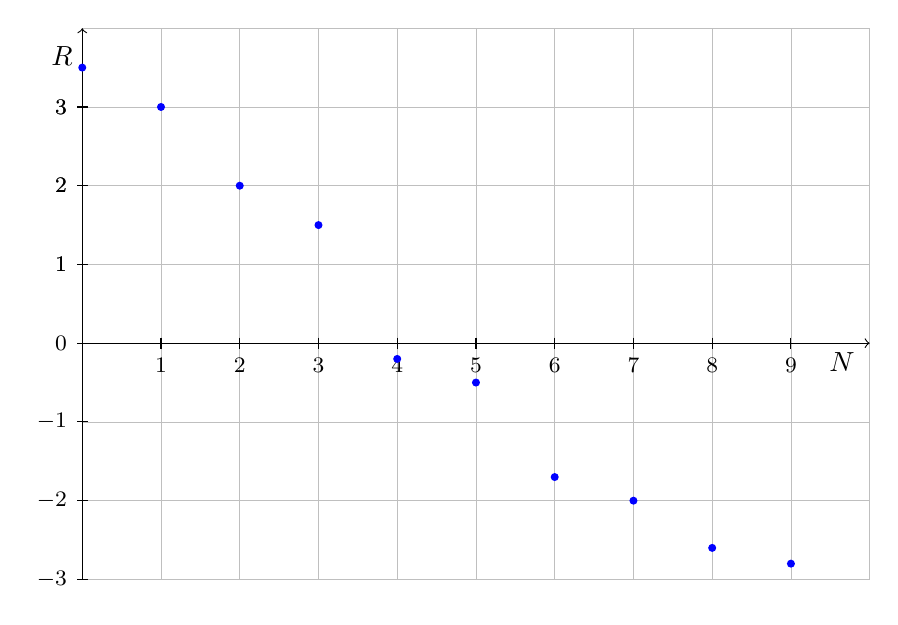
\begin{tikzpicture}
	%\filldraw [red,opacity=0.5] (0,0)--(-1,2)--(-2,4)--(-4,4)--(-4,0)--(0,0);
	% Gitternetzlinien
	\draw[xstep=1cm, ystep=1cm, very thin, color=lightgray] (0,-3) grid (10,4);
	% x-Achse
	\draw[->] (0,0) -- (10,0) node[below,xshift=-1em] {$\mathbb{N}$}; 
	%Zahlen auf x-Achse
	%\foreach \x in {-3,...,-1}
	%\draw[shift={(\x,0)},color=black] (0pt,2pt) -- (0pt,-2pt) node[below] {\footnotesize $\x$};
	\foreach \x in {1,...,9}
	\draw[shift={(\x,0)},color=black] (0pt,2pt) -- (0pt,-2pt) node[below] {\footnotesize $\x$};
	% y-Achse 
	\draw[->] (0,-3) -- (0,4) node[left,yshift=-1em] {$\mathbb{R}$};%node[above left]
	%Zahlen auf y-Achse
	\foreach \y in {-3,...,3}
	\draw[shift={(0,\y)},color=black] (2pt,0pt) -- (-2pt,0pt) node[left] {\footnotesize $\y$};
	\foreach \y in {1,...,3}
	\draw[shift={(0,\y)},color=black] (2pt,0pt) -- (-2pt,0pt) node[left] {\footnotesize $\y$};
	%Ursprung
	%\draw[color=black] (-1.5pt,-2pt) node[below] {\footnotesize $0$};
	
	%\draw[thick,color=black] plot[samples=200, domain=-2:0] 
	%(\x,{-2*\x}) node[below, xshift=-6.5em, yshift=9em] {$y=-2x$};
	
	
	
	\fill [blue] (0,3.5) circle (.051cm) ;	
	
	\fill [blue] (1,3) circle (.051cm) ;
	\fill [blue] (2,2) circle (.051cm) ;
	\fill [blue] (3,1.5) circle (.051cm) ;
	\fill [blue] (4,-0.2) circle (.051cm) ;
	\fill [blue] (5,-0.5) circle (.051cm) ;
	\fill [blue] (6,-1.7) circle (.051cm) ;
	\fill [blue] (7,-2) circle (.051cm) ;
	\fill [blue] (8,-2.6) circle (.051cm) ;
	\fill [blue] (9,-2.8) circle (.051cm) ;	
	%\fill [blue] (8,3) node{\footnotesize streng monoton wachsend} ;	
	\end{tikzpicture}\\
\end{center}
\begin{center}
	Monoton fallende Folge $ (x)_{n\in\mathbb{N}}$\\
	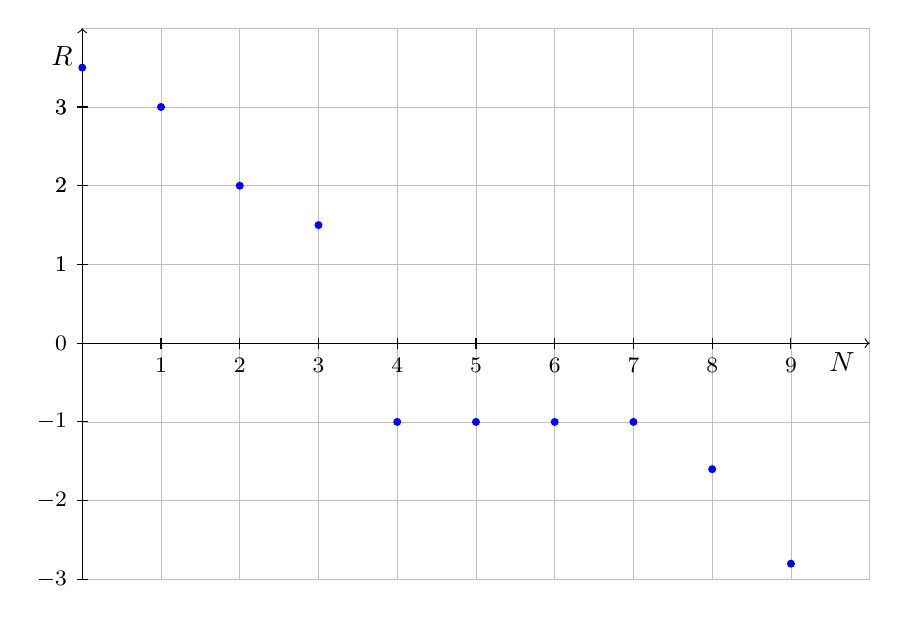
\begin{tikzpicture}
	%\filldraw [red,opacity=0.5] (0,0)--(-1,2)--(-2,4)--(-4,4)--(-4,0)--(0,0);
	% Gitternetzlinien
	\draw[xstep=1cm, ystep=1cm, very thin, color=lightgray] (0,-3) grid (10,4);
	% x-Achse
	\draw[->] (0,0) -- (10,0) node[below,xshift=-1em] {$\mathbb{N}$}; 
	%Zahlen auf x-Achse
	%\foreach \x in {-3,...,-1}
	%\draw[shift={(\x,0)},color=black] (0pt,2pt) -- (0pt,-2pt) node[below] {\footnotesize $\x$};
	\foreach \x in {1,...,9}
	\draw[shift={(\x,0)},color=black] (0pt,2pt) -- (0pt,-2pt) node[below] {\footnotesize $\x$};
	% y-Achse 
	\draw[->] (0,-3) -- (0,4) node[left,yshift=-1em] {$\mathbb{R}$};%node[above left]
	%Zahlen auf y-Achse
	\foreach \y in {-3,...,3}
	\draw[shift={(0,\y)},color=black] (2pt,0pt) -- (-2pt,0pt) node[left] {\footnotesize $\y$};
	\foreach \y in {1,...,3}
	\draw[shift={(0,\y)},color=black] (2pt,0pt) -- (-2pt,0pt) node[left] {\footnotesize $\y$};
	%Ursprung
	%\draw[color=black] (-1.5pt,-2pt) node[below] {\footnotesize $0$};
	
	%\draw[thick,color=black] plot[samples=200, domain=-2:0] 
	%(\x,{-2*\x}) node[below, xshift=-6.5em, yshift=9em] {$y=-2x$};
	
	
	
	\fill [blue] (0,3.5) circle (.051cm) ;	
	
	\fill [blue] (1,3) circle (.051cm) ;
	\fill [blue] (2,2) circle (.051cm) ;
	\fill [blue] (3,1.5) circle (.051cm) ;
	\fill [blue] (4,-1) circle (.051cm) ;
	\fill [blue] (5,-1) circle (.051cm) ;
	\fill [blue] (6,-1) circle (.051cm) ;
	\fill [blue] (7,-1) circle (.051cm) ;
	\fill [blue] (8,-1.6) circle (.051cm) ;
	\fill [blue] (9,-2.8) circle (.051cm) ;	
	%\fill [blue] (8,3) node{\footnotesize streng monoton wachsend} ;	
	\end{tikzpicture}\\
\end{center}
\newpage
\noindent
\begin{center}
	Monoton wachsende Folge $ (x)_{n\in\mathbb{N}}$\\
	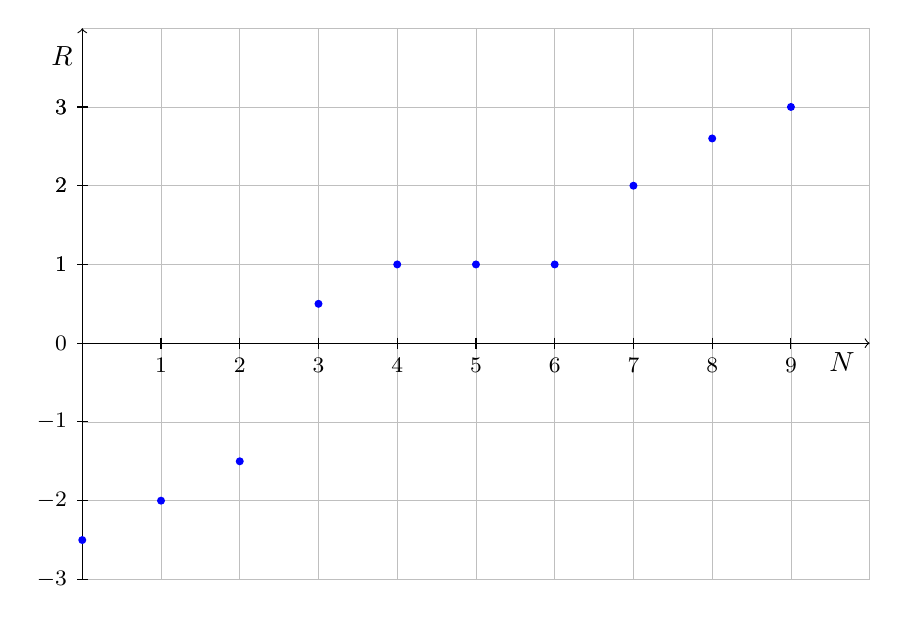
\begin{tikzpicture}
	%\filldraw [red,opacity=0.5] (0,0)--(-1,2)--(-2,4)--(-4,4)--(-4,0)--(0,0);
	% Gitternetzlinien
	\draw[xstep=1cm, ystep=1cm, very thin, color=lightgray] (0,-3) grid (10,4);
	% x-Achse
	\draw[->] (0,0) -- (10,0) node[below,xshift=-1em] {$\mathbb{N}$}; 
	%Zahlen auf x-Achse
	%\foreach \x in {-3,...,-1}
	%\draw[shift={(\x,0)},color=black] (0pt,2pt) -- (0pt,-2pt) node[below] {\footnotesize $\x$};
	\foreach \x in {1,...,9}
	\draw[shift={(\x,0)},color=black] (0pt,2pt) -- (0pt,-2pt) node[below] {\footnotesize $\x$};
	% y-Achse 
	\draw[->] (0,-3) -- (0,4) node[left,yshift=-1em] {$\mathbb{R}$};%node[above left]
	%Zahlen auf y-Achse
	\foreach \y in {-3,...,3}
	\draw[shift={(0,\y)},color=black] (2pt,0pt) -- (-2pt,0pt) node[left] {\footnotesize $\y$};
	\foreach \y in {1,...,3}
	\draw[shift={(0,\y)},color=black] (2pt,0pt) -- (-2pt,0pt) node[left] {\footnotesize $\y$};
	%Ursprung
	%\draw[color=black] (-1.5pt,-2pt) node[below] {\footnotesize $0$};
	
	%\draw[thick,color=black] plot[samples=200, domain=-2:0] 
	%(\x,{-2*\x}) node[below, xshift=-6.5em, yshift=9em] {$y=-2x$};
	
	
	
	\fill [blue] (0,-2.5) circle (.051cm) ;	
	
	\fill [blue] (1,-2) circle (.051cm) ;
	\fill [blue] (2,-1.5) circle (.051cm) ;
	\fill [blue] (3,.5) circle (.051cm) ;
	\fill [blue] (4,1) circle (.051cm) ;
	\fill [blue] (5,1) circle (.051cm) ;
	\fill [blue] (6,1) circle (.051cm) ;
	\fill [blue] (7,2) circle (.051cm) ;
	\fill [blue] (8,2.6) circle (.051cm) ;
	\fill [blue] (9,3) circle (.051cm) ;	
	%\fill [blue] (8,3) node{\footnotesize streng monoton wachsend} ;	
	\end{tikzpicture}\\
\end{center}
\begin{center}
	Monoton wachsende oder fallende Folge $ (1)_{n\in\mathbb{N}}$\\
	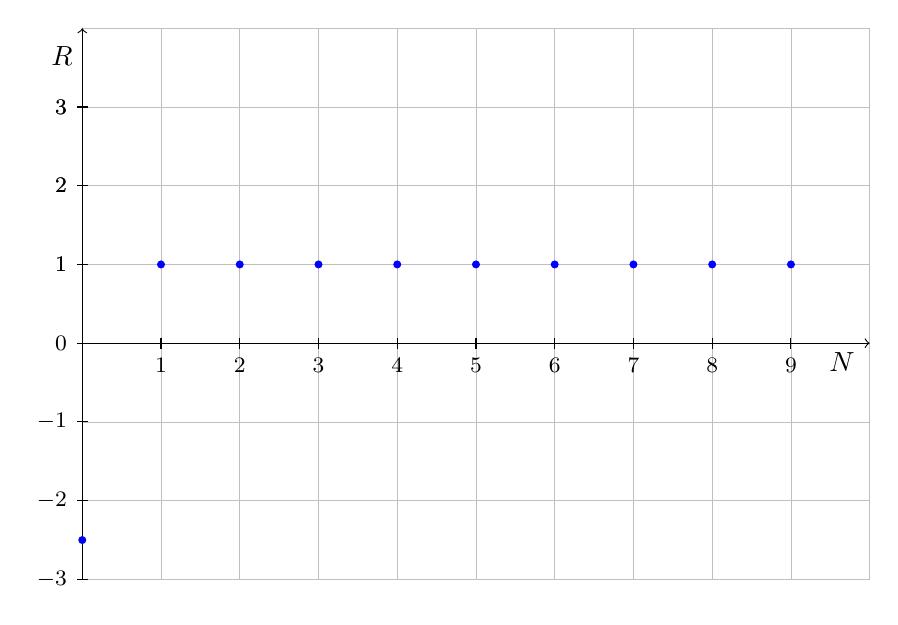
\begin{tikzpicture}
	%\filldraw [red,opacity=0.5] (0,0)--(-1,2)--(-2,4)--(-4,4)--(-4,0)--(0,0);
	% Gitternetzlinien
	\draw[xstep=1cm, ystep=1cm, very thin, color=lightgray] (0,-3) grid (10,4);
	% x-Achse
	\draw[->] (0,0) -- (10,0) node[below,xshift=-1em] {$\mathbb{N}$}; 
	%Zahlen auf x-Achse
	%\foreach \x in {-3,...,-1}
	%\draw[shift={(\x,0)},color=black] (0pt,2pt) -- (0pt,-2pt) node[below] {\footnotesize $\x$};
	\foreach \x in {1,...,9}
	\draw[shift={(\x,0)},color=black] (0pt,2pt) -- (0pt,-2pt) node[below] {\footnotesize $\x$};
	% y-Achse 
	\draw[->] (0,-3) -- (0,4) node[left,yshift=-1em] {$\mathbb{R}$};%node[above left]
	%Zahlen auf y-Achse
	\foreach \y in {-3,...,3}
	\draw[shift={(0,\y)},color=black] (2pt,0pt) -- (-2pt,0pt) node[left] {\footnotesize $\y$};
	\foreach \y in {1,...,3}
	\draw[shift={(0,\y)},color=black] (2pt,0pt) -- (-2pt,0pt) node[left] {\footnotesize $\y$};
	%Ursprung
	%\draw[color=black] (-1.5pt,-2pt) node[below] {\footnotesize $0$};
	
	%\draw[thick,color=black] plot[samples=200, domain=-2:0] 
	%(\x,{-2*\x}) node[below, xshift=-6.5em, yshift=9em] {$y=-2x$};
	
	
	
	\fill [blue] (0,-2.5) circle (.051cm) ;	
	
	\fill [blue] (1,1) circle (.051cm) ;
	\fill [blue] (2,1) circle (.051cm) ;
	\fill [blue] (3,1) circle (.051cm) ;
	\fill [blue] (4,1) circle (.051cm) ;
	\fill [blue] (5,1) circle (.051cm) ;
	\fill [blue] (6,1) circle (.051cm) ;
	\fill [blue] (7,1) circle (.051cm) ;
	\fill [blue] (8,1) circle (.051cm) ;
	\fill [blue] (9,1) circle (.051cm) ;	
	%\fill [blue] (8,3) node{\footnotesize streng monoton wachsend} ;	
	\end{tikzpicture}\\
\end{center}
Beispiel:\\
\textbullet \;\; Die Folge $ (n)_{n\in\mathbb{N}} $ ist streng monoton wachsend, weil:\\
\begin{align*}
x_n=n< x_{n+1}=n+1 \;\;\text{für alle }\;\;n\in\mathbb{N}
\end{align*}
\textbullet \;\;Die Folge $ (\frac{1}{n})_{n\in\mathbb{N}\backslash\{0\}} $ ist streng monoton fallend, weil:\\
\begin{align*}
x_n=\frac{1}{n}>x_{n+1}=\frac{1}{n+1}\;\;\text{für alle } n\in\mathbb{N}\backslash\{0\}
\end{align*}
\textbullet \;\; Die konstante Folge $ (a)_{n\in \mathbb{N}} $ mit  $ a\in\mathbb{R} $ ist sowohl monoton wachsend als auch monoton fallend.\\
\subsubsection{Aufgabe zur Monotonie von Folgen}
\href{https://youtu.be/WSqcscE6Dhg}{Video 14}\\
Zeige, dass dir rekrusive Folge gegeben durch $a_0=1,\; a_{n+1}=a_n+\frac{1}{a_n} $ streng monoton wachsend ist.\vspace*{2mm}\\
Bemerkung:\\
Bei einer rekrusiven Folge muss man die Monotonie mit Hilfe der vollständigen Induktion beweisen.\\
Die Summanden von der rekrusiven Folge müssen größer Null sein, dass die streng wachsende Monotonie möglich ist.\\
Also zeige:\\
\begin{align*}
a_n>0 \;\;\text{für alle }\;\;n_0\in \mathbb{N}\Rightarrow \frac{1}{a_n}>0
\end{align*}
Damit hätte man:\\
\begin{align*}
&a_{n+1}=a_n+\frac{1}{a_n}>a_n+0=a_n \;\;\text{für alle }\;\;n\in \mathbb{N}\\
&a_{n+1}> a_n
\end{align*}
Beweis von $ a_n>0 $ für alle $ n\in\mathbb{N} $ mittels vollständiger Induktion:\\
\textbf{\textbullet \;\; (I.A.)}:\\
\begin{quote}
	für $ n=0 $ gilt:\\
	\begin{align*}
	a_n=a_0=1>0_{\;\;_{\Square}}
	\end{align*}
\end{quote}
\textbf{\textbullet \;\; (I.V.)}:\\
\begin{quote}
	für ein $ n $ gilt:\\
	\begin{align*}
	a_n>0 \Rightarrow \frac{1}{a_n}>0
	\end{align*}
\end{quote}
\textbf{\textbullet \;\;(I.S.)}:\\
\begin{quote}
	zu zeigen:\\
	\begin{align*}
	a_{n+1}>0
	\end{align*}
	betrachte:\\
	\begin{align*}
	a_{n+1}>a_n+\frac{1}{a_n}\overset{(I.V.)}{>}0+ 0=0_{\;\;_{\Square}}
	\end{align*}
\end{quote}
\newpage
\noindent
\subsection{Beschränktheit von Folgen }
\href{https://youtu.be/ftHUnCyM89E}{Video 15}\\
Die reelle Folge $ (x)_{n\in\mathbb{N}} $ heißt beschränkt, wenn es $ a,b \in \mathbb{R} $ gibt mit $ a\leq x_n\leq b $ für alle $ n\in \mathbb{N} $\\
\begin{center}
	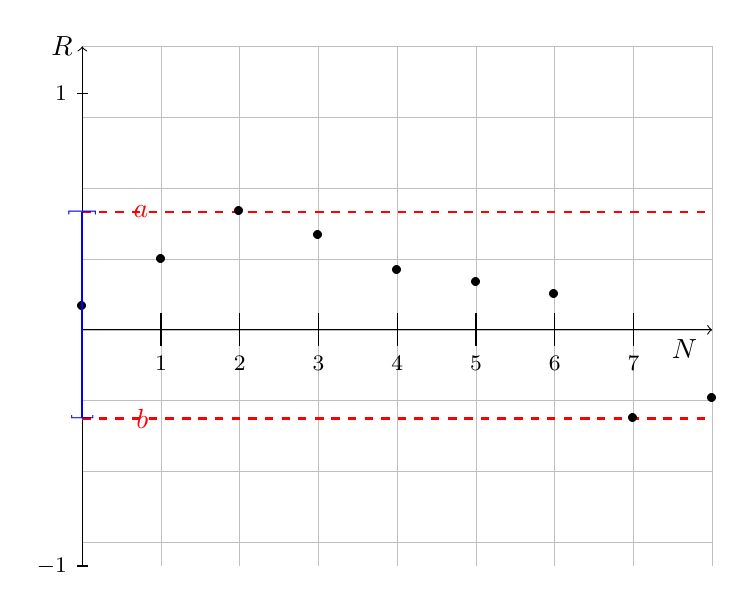
\begin{tikzpicture}[yscale=3]
	
	% Gitternetzlinien
	\draw[xstep=1cm, ystep=0.3cm, very thin, color=lightgray] (0,-1) grid (8,1.2);
	% x-Achse
	\draw[->] (0,0) -- (8,0) node[below,xshift=-1em] {$\mathbb{N}$}; 
	%Zahlen auf x-Achse
	\foreach \x in {1,...,7}
	\draw[shift={(\x,0)},color=black] (0pt,2pt) -- (0pt,-2pt) node[below] {\footnotesize $\x$};
	%\foreach \x in {1,...,3}
	%\draw[shift={(\x,0)},color=black] (0pt,2pt) -- (0pt,-2pt) node[below] {\footnotesize $\x$};
	% y-Achse 
	\draw[->] (0,-1) -- (0,1.2) node[left,yshift=0em] {$\mathbb{R}$};%node[above left]
	%Zahlen auf y-Achse
	\foreach \y in {-1,...,-1}
	\draw[shift={(0,\y)},color=black] (2pt,0pt) -- (-2pt,0pt) node[left] {\footnotesize $\y$};
	\foreach \y in {1,...,1}
	\draw[shift={(0,\y)},color=black] (2pt,0pt) -- (-2pt,0pt) node[left] {\footnotesize $\y$};
	%Ursprung
	%\draw[color=black] (0pt,-10pt) node[right] {\footnotesize $0$};
	
	\draw[thick,color=red,dashed] plot[samples=200, domain=0:8] 
	(\x,{1/2}) node[left, xshift=-20em] {$a$};
	
	\draw[thick,color=red,dashed] plot[samples=200, domain=0:8] 
	(\x,{-1.5/4}) node[left, xshift=-20em]{$b$};
	\draw[color=black] (0,0.1) node {\footnotesize \textbullet};
	\draw[color=blue,thick] (0,-1.5/4) --(0,0.5);
	\draw[color=blue,thick] (0,-1.5/4) node[rotate=90] {\footnotesize $[$};
	\draw[color=blue,thick] (0,0.5) node[rotate=90] {\textbf{$]$}};
	\draw[color=black] (1,0.3) node {\footnotesize \textbullet};
	\draw[color=black] (2,0.5) node {\footnotesize \textbullet};
	\draw[color=black] (3,0.4) node {\footnotesize \textbullet};
	\draw[color=black] (4,0.25) node {\footnotesize \textbullet};
	\draw[color=black] (5,0.2) node {\footnotesize \textbullet};
	\draw[color=black] (6,0.15) node {\footnotesize \textbullet};
	\draw[color=black] (7,-1.5/4) node {\footnotesize \textbullet};
	\draw[color=black] (8,-0.29) node {\footnotesize \textbullet};
	
	%\draw[color=black] (-1.5,0) node {\footnotesize Grenzwert=0};
	%\draw[color=black] (5,-0.4) node {\footnotesize $ n_0=5 $};
	\end{tikzpicture}\\
\end{center}
\begin{align*}
\Leftrightarrow x_n\in [a,b]\;\;\text{für }\;\; n\in \mathbb{N}
\end{align*}
Beispiel:\\
\textbullet \;\; Die Folge $ \big((-1)^n\big)_{n\in\mathbb{N}} $ ist beschränkt weil:\\
\begin{quote}
	\begin{align*}
	-1\leq(-1)^n\leq 1\;\;\text{für alle }\;\; n\in\mathbb{N}\\
	-20\leq(-1)^n\leq 20\;\;\text{für alle }\;\; n\in\mathbb{N}\\
	(-1)^n \in [-200,15]\\
	\end{align*}
	Kleinste obere Schranke oder obere Schanke, bzw. größte untere Schranke oder untere Schranke. Wichtig ist eigentlich ist die Folge beschränkt oder nicht.\\
	Bemerkung:\\
	\begin{align*}
	(-1)^n \;\;\text{ist nicht konvergent, aber beschränkt ! }
	\end{align*}
\end{quote}
\textbullet \;\;Die Folge $ (\frac{1}{n}) $ ist beschränkt weil:\\
\begin{quote}
	\begin{align*}
	1\geq \frac{1}{n}\geq 0 \;\;\text{für alle }\;\;n\in\mathbb{N}_{\backslash\{0\}}
	\end{align*}
\end{quote}
\textbullet \;\; Die Folge $ (n)_{n\in\mathbb{N}} $ ist unbeschränkt, weil:\\
\begin{quote}
	Es gibt eine untere Schranke, aber keine obere Schranke.\\
	\begin{align*}
	x_n=n\in[0,\infty[
	\end{align*}
\end{quote}
\subsubsection{Aufgabe zur Beschränktheit von Folgen }
\href{https://youtu.be/w8bu4mqcZrQ}{Video 16}\\
Zeige, dass die rekrusive Folge, gegeben durch $ a_0=0 $ und $ a_{n+1}=\frac{1}{3}(a_n+1)$ für alle $ n\in \mathbb{N} $ durch $ 0 $ und $ 1 $ beschränkt ist.\vspace*{2mm}\\
Zu zeigen:\\
\begin{align*}
0\leq a_n < 1 \;\;\text{für alle }\;\;n\in \mathbb{N}
\end{align*}
Beweis mittels vollständiger Induktion.\\
\textbf{\textbullet \;\; (I.A.):}\\
\begin{quote}
	für $ n=0 $ gilt:\\
	\begin{align*}
	a_n=0=a_0=0\;\;\in[0,1 [_{\;\;_{\Square}}
	\end{align*}
	
\end{quote}
\textbf{\textbullet \;\; (I.V.):}\\
\begin{quote}
	für ein $ n\in\mathbb{N} $ gilt:\\
	\begin{align*}
	0\leq a_n < 1
	\end{align*}
\end{quote}
\textbf{\textbullet \;\; (I.S.):}\\
\begin{quote}
	zu zeigen:\\
	\begin{align*}
	0\leq a_{n+1} < 1
	\end{align*}
	Betrachte für $ a_n<1 $\\
	\begin{align*}
	a_{n+1}=\frac{1}{3}(a_n+1)=\frac{1}{3}a_n+\frac{1}{3}\overset{(I.V.)}{<}\frac{1}{3}\cdot1 +\frac{1}{3}=\frac{2}{3}<1_{\;\;_{\Square}}\\
	\end{align*}
	Betrachte für $ a_n\geq 0 $\\
	\begin{align*}
	&a_{n+1}=\frac{1}{3}(a_n+1)=\frac{1}{3}a_n+\frac{1}{3}\overset{(I.V.)}{>}\frac{1}{3}\cdot 0 +\frac{1}{3}>0_{\;\;_{\Square}}\\
	&a_{n+1}\geq 0 \;\;\text{weil $ a_{n_{0}}=0=a_0 $, deswegen: $ \geq $ }
	\end{align*}
	\begin{align*}
	\Rightarrow 0\leq a_{n+1} < 1
	\end{align*}
\end{quote}
\subsection{Konvergenzkriterien }
\href{https://youtu.be/KU9z0fJVi-U}{Video 17}\\
Konvergenzkriterium:\\
\begin{center}
	
	
	\fbox{\parbox  {120mm} {
			Jede monotone und beschränkte Folge reeller Zahlen ist konvergent.}}
\end{center}
Beispiel:\\
\textbullet \;\; Die Folge $ (\frac{1}{n})_{n\in\mathbb{N}\backslash\{0\}} $:\\
\begin{quote}
	(i) Monotonie:\\
	\begin{quote}
		Die Folge ist streng monoton fallend, da:\\
		\begin{align*}
		x_n=\frac{1}{n}>\frac{1}{n+1}=x_{n+1} \;\;\text{für alle}\;\;n\in\mathbb{N}{\backslash\{0\}}
		\end{align*}
	\end{quote}
	(ii) Beschränktheit:\\
	\begin{quote}
		Die Folge ist beschränkt, da:\\
		\begin{align*}
		0<\frac{1}{n}\leq 1 \;\;\text{für alle }n\in\mathbb{N}{\backslash\{0\}}
		\end{align*}
	\end{quote}
	Weil die Folge monoton und beschränkt ist, ist die Folge konvergent.\\
	Bemerkung:\\
	Die Folge ist immer größer als Null, aber der Grenzwert $ \lim\limits_ {n\to\infty} \frac{1}{n}=0 $.
	
\end{quote}
\textbullet \;\; Die Folge $ \bigg(\frac{(-1)^n}{n}\bigg)_{n\in\mathbb{N}\backslash\{0\}} $\\
\begin{quote}
	(i) Monotonie\\
	\begin{quote}
		Die Folge ist nicht monoton, da:\\
		\begin{align*}
		&\bigg(\frac{(-1)^n}{n}\bigg)_{n\in\mathbb{N}\backslash\{0\}}=-1,\frac{1}{2},-\frac{1}{3}\ldots\\
		&-1<\frac{1}{2}>-\frac{1}{3}\\&\Rightarrow \;\;\text{Die Folge ist schon nach drei Glieder nicht monoton. }
		\end{align*}
	\end{quote}
	(ii) Beschränktheit:\\
	\begin{quote}
		Die Folge ist beschränkt, da:\\
		\begin{align*}
		-1\leq \frac{(-1)^n}{n}<1\;\;\text{für alle }\;\;n\in\mathbb{N}\backslash\{0\}
		\end{align*}
		Aber: Der Grenzwert der Folge ist:\\
		\begin{align*}
		\lim\limits_ {n\to\infty} \frac{(-1)^n}{n}=0
		\end{align*}
		Deshalb ist diese Folge konvergent.\\
	\end{quote}
\end{quote}
Fazit:\\
Monotonie $ + $ Beschränktheit $ \Rightarrow $ Konvergenz\\
Aber nicht:\\
Konvergenz $ \nRightarrow $ Monotonie $ + $ Beschränktheit\\
\subsubsection{Aufgabe zum Konvergenzkriterien-Teil I}
\href{https://youtu.be/fpaipwCojak}{Video 18}\\
Beweise, dass die rekrusive Folge gegeben durch $ x_0=\sqrt{3} $ und $ x_{n+1}=\sqrt{3+x_n} $ \;für alle $ n\in \mathbb{N} $ konvergiert und berechne, wenn vorhanden, den Grenzwert.\\
Vorgehensweise bei der Lösung:\\
\begin{tabular}[t]{ll}% l=linksbündig r=rechtsbündig
	(i) & Nachweis der Monotonie  \\
	(ii) & Nachweis der Beschränktheit\\
	(iii) & Grenzwert berechnen \\	
\end{tabular} \\
\\
(i)\;\;Nachweis der Monotonie\\
\begin{quote}
	Zuerst einfach Zahlen in die Folge $ x_{n+1}=\sqrt{3+x_n} $ einsetzen.\\
	Dies ergibt:\\
	$x_0=\sqrt{3}$\\
	$x_1=\sqrt{3+\sqrt{3}}$\\
	$x_2=\sqrt{3+\sqrt{3+\sqrt{3}}}$\\
	Da die Wurzel immer positiv ist, wird die Folge streng monoton steigend sein.\\
	Zu zeigen:
	\begin{align*}
	x_n<x_{n+1}\;\;\text{für alle }\;\;n\in\mathbb{N}
	\end{align*}
	Beweis mt vollständiger Induktion:\\
	\textbullet \;\;\textbf{(I.A.):}\\
	\begin{quote}
		für $ n=0$ gilt:\\
		\begin{align*}
		x_0=\sqrt{3}<x_{n+1}=x_1=\sqrt{3+\sqrt{3}}_{\;\;_{\Square}}
		\end{align*}
	\end{quote}
	\textbullet \;\;\textbf{(I.V.):}\\
	\begin{quote}
		für ein $ n\in\mathbb{N} $ gilt:\\
		\begin{align*}
		x_{n+1}>x_{n}
		\end{align*}
	\end{quote}
	\textbullet \;\;\textbf{(I.S.):}\\
	\begin{align*}
	x_{n+2}>x_{n+1}
	\end{align*}
	Betrachte:
	\begin{align*}
	x_{n+2}=\sqrt{3+\sqrt{x_{n+1}}}\overset{(I.V.)}{\geq}\sqrt{3+x_n}=x_{n+1_{\;\;\Square}}
	\end{align*}
	Die Folge ist streng monoton steigend.
\end{quote}





\subsubsection{Aufgabe zum Konvergenzkriterien-Teil II}
\href{https://youtu.be/ldMJJfYpobk}{Video 19}\\
(ii)\;\;Nachweis der Beschränktheit\\
\begin{quote}
	Zu zeigen:\\
	Es gibt $ a,b\in\mathbb{R} $ mit $ a\leq x_n\leq b $ für alle $ n\in\mathbb{N} $\vspace*{2mm}\\
	Es gilt:\\
	$ x_n $ ist streng monoton wachsen, d.h. $ x_n<x_{n+1} $ oder $ x_0<x_1<x_2\ldots $\\
	Es gilt also für $ x_0=\sqrt{3} $:\\
	\begin{align*}
	\sqrt{3}\leq x_n\;\;\text{für alle }\;\;n\in\mathbb{N}\\
	\Rightarrow a=\sqrt{3} \;\;\text{ist untere Schranke }
	\end{align*}
	Die obere Schranke muss man durch Ausprobieren einfach abschätzen.\\
	Es soll gelten: $ x_n<10 $\\
	Beweis mit vollständiger Induktion:\\
	\textbullet \;\;(I.A.):\\
	\begin{quote}
		für $ n=0 $ gilt:\\
		\begin{align*}
		x_0=\sqrt{3}<10_{\;\;_{\Square}}
		\end{align*}
	\end{quote}
	
	\textbullet \;\;(I.V.):\\
	\begin{quote}
		für ein $ n\in\mathbb{N} $ gilt:\\
		\begin{align*}
		x_{n+1}=\sqrt{3+x_n}<10
		\end{align*}
	\end{quote}
	\textbullet \;\;(I.S.):\\
	\begin{quote}
		\begin{align*}
		x_{n+2}=\sqrt{3+x_{n+1}}<10
		\end{align*}
		Betrachte:\\
		\begin{align*}
		x_{n+2}=\sqrt{3+x_{n+1}}\overset{(I.V.)}{<} \sqrt{3+10}=\sqrt{13}<10_{\;\;_{\Square}}
		\end{align*}
		\begin{align*}
		&\Rightarrow b=10\;\;\text{ ist eine obere Schranke}\\
		&\Rightarrow a=\sqrt{3}\;\;\text{ ist eine untere Schranke}\\
		&\text{Es gilt für}\;\;a,b \in \mathbb{R} \;\;a\leq x_n< b\;\;\text{für alle }\;\;n\in\mathbb{N}
		\end{align*}
	\end{quote}
	Fazit:\\
	Die Folge ist beschränkt, außerdem ist sie streng monoton wachsend, daraus folgt mit dem Konverkenzkriterium, dass die Folge konvergent ist.
\end{quote}


\subsubsection{Aufgabe zum Konvergenzkriterien-Teil III}
\href{https://youtu.be/4zIPa5nNbdU}{Video 20}\\
(iii)\;\;Grenzwert berechnen\\
\begin{quote}
	Die Folge mit $ x_0=\sqrt{3} $ und $ x_{n+1}=\sqrt{3+x_n} $ für alle $ n\in\mathbb{N} $ ist konvergent.\vspace*{4mm}\\
	Bemerkung:\\
	\begin{quote}
		Es gilt:\\
		\begin{align*}
		(a_n)_{n\in\mathbb{N}}\;\;\text{konvergiert gegen } \;\;a\\
		\end{align*}
		Dann gilt auch:\\
		\begin{align*}
		\lim\limits_ {n\to\infty}a=\lim\limits_ {n\to\infty}a_{n+1}
		\end{align*}
		Beispiel:\\
		\begin{align*}
		\lim\limits_ {n\to\infty}\frac{1}{n}=\lim\limits_ {n\to\infty}\frac{1}{n+1}=0
		\end{align*}
		Das heißt:\\
		\begin{align*}
		\lim\limits_ {n\to\infty}x_n=a=	\lim\limits_ {n\to\infty}x_{n+1}\;\;\text{für } \;\;a=\in\mathbb{R}\\
		\end{align*}
	\end{quote} 
	Für die Folge gilt dann:\\
	\begin{align*}
	\lim\limits_ {n\to\infty}\sqrt{3+x_n}=a\\
	\Leftrightarrow a=\sqrt{3+a}
	\end{align*}
	Berachte also:\\
	\begin{align*}
	\sqrt{3+a}=a\Leftrightarrow 0&=a^2-a-3\\
	&=a^2-a+\frac{1}{4}-\frac{1}{4}-3\\
	&=\bigg(a-\frac{1}{2}\bigg)^2-\frac{13}{4}\\
	\Leftrightarrow \bigg(a-\frac{1}{2}\bigg)^2&=\frac{13}{4}\\
	\Leftrightarrow a_{1,2}&=\frac{1}{2}\pm \sqrt{\frac{13}{4}}=\frac{1}{2}\pm \frac{\sqrt{13}}{2}=\frac{1\pm\sqrt{13}}{2}
	\end{align*}
	Die Folge ist streng monoton wachsend $ (\sqrt{3}\leq x_n\;\;\text{für alle }\;\;n\in\mathbb{N}) $ , also kann die Lösung nur positiv sein.\\
	Deshalb gilt für den Grenzwert:\\
	\begin{align*}
	a=\frac{1+\sqrt{13}}{2}
	\end{align*}
	
\end{quote}


